\documentclass{article}
\usepackage{graphicx}
\usepackage[margin=1in]{geometry}
\usepackage{amsmath}
\title{Mathematical Modeling Project}
\author{Tyler Lukasiewicz, Liana Severo, Caitlin Buttery}
\begin{document}
\maketitle
\abstract{
Here I am changing something i am belle lololol mea quidam pericula appellantur, ne quo vitae recteque. Duo ullum deserunt definitiones ea, ex has vocent constituam inciderint, at novum philosophia has. Summo facete audire eu pro, mazim tritani tibique ne quo. Justo deterruisset reprehendunt qui cu, nam te debet oblique incorrupte. Usu nominavi copiosae patrioque et, nec ferri constituto ei.

}
\section{Introduction}
\label{sec:Introduction}
Lorem ipsum dolor sit amet, id mea quidam pericula appellantur, ne quo vitae recteque. Duo ullum deserunt definitiones ea, ex has vocent constituam inciderint, at novum philosophia has. Summo facete audire eu pro, mazim tritani tibique ne quo. Justo deterruisset reprehendunt qui cu, nam te debet oblique incorrupte. Usu nominavi copiosae patrioque et, nec ferri constituto ei.


\section{Research and Methods}
\label{sec:Main part}

\subsection{Immune System Response to a Single Viral Strain}
\begin{equation}
    \begin{split}
        \dot v &= v(r-ax) = f_1(v,x), \\
        \dot x &= -bx + cv = f_2(v,x)
    \end{split}
\end{equation}

Here, $v$ is the viral strain. $x$ is the specific immune system response to the strain. $r$ is the rate at which the virus reproduces. $a$ is the rate at which the immune cells destroy the virus. $b$ is the rate at which the immune cells die off. $c$ is rate at which the immune cells reproduce, which is dependent on the number of viruses present, $v$.  
\subsubsection{Getting our eigenvalues}
First we take the Jacobian matrix of our system, which is
\begin{equation}
    J =
    \begin{pmatrix}
        r-ax    & -av \\
        c       & -b
    \end{pmatrix}
\end{equation}
Then we find the characteristic equations by evaluating the Jacobian at the two fixed points of our system $(0,0)$ and $(\alpha,\beta)$, where $\alpha = \frac{br}{ac} $ and let $\beta = \frac{r}{a} $
\begin{equation}
    \begin{split}
        &J(0,0) - \lambda I = \lambda^2 + \lambda(b-r) -br = 0\\
        &\implies \lambda_{1,2} = r,-b\\
        &J(\alpha,\beta)  - \lambda I =  \lambda^2 + \lambda \gamma + \delta\\ 
        &\implies \lambda_{1,2} = \frac{-\gamma \pm \sqrt{\gamma^2 - 4\delta}}{2} \\
        \text{where} \\
        &\gamma =  b - r + a\beta \text{, and } \delta = ac\alpha + ab\beta -rb
    \end{split}
\end{equation}
\subsubsection{Modeling the System With One Viral Strain}
We will now model our system of equations with conditions $r = 2.4, a = 2, b = 0.1, \text{ and }c = 1.$. We will also assume that we are starting with no viruses and no immune response.
\label{sub:modeling the sytem}

The fixed point $(0,0)$ corresponds to the eigenvalues $\lambda_1 = 2.4, \lambda_2 = -.1$, which implies that $(0,0)$ is a saddle point. The fixed point $(\alpha,\beta) = (.12,1.2)$ results in eigenvalues $\lambda_1 = -.05 + 4.873i , \lambda_2 = -.05 - 4873i$, which implies that the point $(.12,1.2)$ is a spiral sink. So in this system both the viral strain and immune response will begin oscillating dramatically and then as time approaches infinity, they will settle to stable values. This is illustrated in figure \ref{fig:hiv1}
\label{sub:Determining Stability of Fixed points}
\begin{figure}[h!]
    \centering
    \caption{\textbf{\textit{Population size of the viral load and the immune response for a single virus strain with r = 2.4, a = 2, b = 0.1, c = 1.}}}
    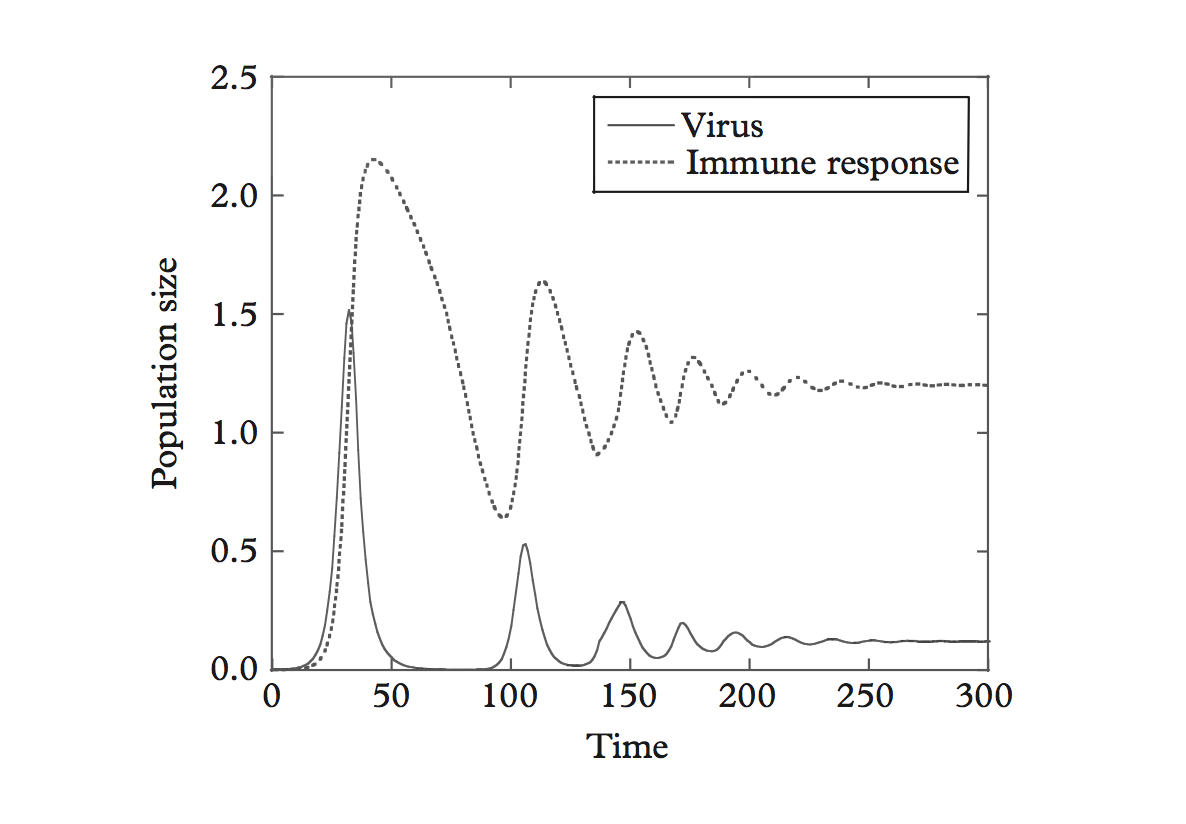
\includegraphics[scale=.4]{imgs/hiv_graph1.png}
    \label{fig:hiv1}
\end{figure}

\subsection{Modeling the System with Multiple Viral Strains}
Suppose there are $N$ strains of the virus.  The $i$th strain of the virus $v_i$ and the immunal reaction $x_i$ to it can be modeled by the system of equations
\begin{equation}
    \begin{split}
        \dot v_i &= v_i(r - ax_i), \\
        \dot x_i &= -bx_i + cv_i
    \end{split}
\end{equation}
This adds a degree of randomness to our behavior, as new viruses can appear at any point in time. We may begin with only one virus, which can proceed to mutate as it pleases, or we may begin with many strains. Each new viral strain should result in a new immune response. Eventually, a global immune response will take care of all $N$ viral strains regardless of mutation or rate of mutation. This global response can be modeled by the system of equations
\begin{equation}
    \begin{split}
        \dot v_i &= v_i(r - ax_i - qz) \\
        \dot x_i &= -bx_i + cv_i \\
        \dot z &= kv - bz
    \end{split}
\end{equation}
Where $z$ is the cross reactive response that decays at rate $b$.  $v = \sum^{N}_{i=1} v_i$ is the total viral load. $q$ is the rate at which the virus evades the global response, and $k$ is the rate at which the global response grows in comparison to the number of preheat viral strains.


\subsubsection{Getting Eigenvalues}
First we take the Jacobian of the system of equations.
%the jacobian
\begin{equation}
    J=
    \begin{pmatrix}
        -ax-qz+r    &-va    &-qv    \\
        c           &-b     &0      \\
        k           &0       &-b
    \end{pmatrix}
\end{equation}
%the characteristic equation
Next we find the characteristic equation
\begin{equation}
    \begin{split}
        J - \lambda I &= \\ 
        &-a{b}^{2}x-abcv-2\,ab\lambda\,x-ac\lambda\,v-a{\lambda}^{2}x-{b}^{2}qz -bkqv-2\,b\lambda\,qz-k\lambda\,qv \\
        &-{\lambda}^{2}qz-{b}^{2}\lambda+{b}^ {2}r-2\,b{\lambda}^{2}+2\,b\lambda\,r-{\lambda}^{3}+{\lambda}^{2}r
    \end{split}
\end{equation}

solving for lambda, we get the eigenvalues

\begin{equation}
    \begin{split}
        \lambda_1 &=  -b\\
        \lambda_2 &= -1/2\,ax-1/2\,qz-b/2+r/2 \\ 
        &+1/2\,\sqrt {{a}^{2}{x}^{2}+2\,axqz+{q}^{2}{z} ^{2}-2\,abx-4\,acv-2\,axr-2\,bqz-4\,kqv-2\,qzr+{b}^{2}+2\,br+{r}^{2}} \\
        \lambda_3 &= -1/2\,ax-1/2\,qz-b/2+r/2 \\ 
        &-1/2\,\sqrt {{a}^{2}{x}^{2}+2\,axqz+{q}^{2}{z} ^{2}-2\,abx-4\,acv-2\,axr-2\,bqz-4\,kqv-2\,qzr+{b}^{2}+2\,br+{r}^{2}}
    \end{split}
\end{equation}


\subsubsection{Modeling The Equation}

\begin{equation}
    \begin{split}
        r = 2.4, a = 2, b=0.1,c=1,q=2.4,k=1
    \end{split}
    \label{eq:vals}
\end{equation}

Evaluating the characteristic equation at the fixed points $\{v = 0,x = 0,z = 0\}$ with the values in \ref{eq:vals} and solving for $\lambda$ we get
\begin{equation}
    \lambda_{1,2,3} = 2.4,-.1,-.1
\end{equation}

So we know that the point $(0,0,0)$ is a source. Now we need to find the interesting part of the equation. Setting our system of equations to zero and solving for $x,v\text{ and } z$ we get the fixed point
%fixed points of equation
\begin{equation}
v ={\frac {br}{ac+kq}},x ={ \frac {cr}{ac+kq}},z={\frac {kr}{ac+kq}}
    \label{eq:fixed}
\end{equation}

Evaluating the characteristic equation at the fixed points in \ref{eq:fixed} with the values in \ref{eq:vals} and solving for $\lambda$ we get
\begin{equation}
    \lambda_{1,2,3} = -.1,-.05 \pm .4873i
\end{equation}
So the fixed point $\{v = .0\overline{54}, x = .\overline{54}, z =.\overline{54}\}$ is a stable spiral. 

\begin{figure}[h!]
    \centering
    \caption{\textbf{\textit{Example of a cross-reactive immune response. The total population sizes of the viral load and the immune response are shown for r = 2.4, a = 2, b=0.1,c=1,q=2.4,k=1 with a random probability for the rise of new virus strains.}}}
    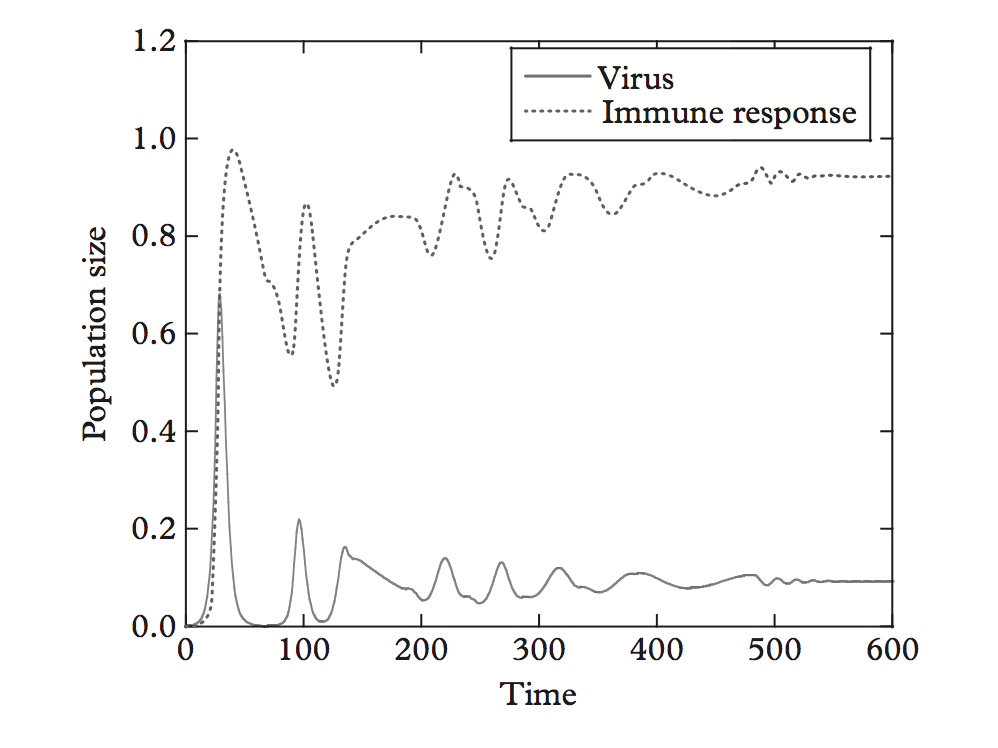
\includegraphics[scale=.4]{imgs/hiv_graph2.png}
    \label{fig:hiv2}
\end{figure}

\subsection{HIV Section}

\subsection{Ebola Section}
Ebola is known to evade the immune system during infection. We present a mathematical model of a system of non-linear ordinary differential equations derived from known biological dynamics and a few biologically reasonable assumptions.

\subsubsection{Ebola Background}
\subsubsection{The Herz Model}
The Herz Model is a deterministic model for viral reproduction, which describes all events using a system of three equations:

	x(t) = number of uninfected cells
	y(t) = number of infected cells
	v(t) = number of free virus particles

And a modification, since contact between a virus and a cell reduces the number of available free virus.

\begin{equation}
	\begin{split}
	dx/dt = lambda - 
	\end{split}
\end{equation}



\section{Conclusion}
\label{sub:Conclusion}
Lorem ipsum dolor sit amet, id mea quidam pericula appellantur, ne quo vitae recteque. Duo ullum deserunt definitiones ea, ex has vocent constituam inciderint, at novum philosophia has. Summo facete audire eu pro, mazim tritani tibique ne quo. Justo deterruisset reprehendunt qui cu, nam te debet oblique incorrupte. Usu nominavi copiosae patrioque et, nec ferri constituto ei.



\begin{thebibliography}{9}
\bibitem{latexcompanion} 
Michel Goossens, Frank Mittelbach, and Alexander Samarin. 
\textit{The \LaTeX\ Companion}. 
Addison-Wesley, Reading, Massachusetts, 1993.
\end{thebibliography}


\end{document}
